\documentclass[a4paper, twocolumn]{article}
\usepackage[utf8]{inputenc}
\usepackage[english]{babel}
\usepackage{graphicx}
\usepackage{wrapfig}
\usepackage{lipsum}
\usepackage{multicol}
\usepackage{hyperref}
\usepackage{enumitem}
\usepackage{float}
\usepackage{tikz}
\usepackage{amsmath}
\usetikzlibrary{shapes, arrows.meta, positioning}
\usepackage[margin=0.5in]{geometry}
\setlength{\parskip}{0.3em}
\setlength{\columnsep}{20pt}
\date{}
\raggedbottom
\raggedcolumns

\title{
\textbf{Carry Trade Shield: A Risk Mitigation Product for Currency and Stock Volatility}\\
Group 2
}

\author{
    Lyu Xing \\
    3035973828 \\
    u35xing@connect.hku.hk
    \and
    Zheng Yiwen \\
    3035844534 \\
    zyw666@connect.hku.hk
    \and
    Tao Chenya \\
    3036303044 \\
    u3630304@connect.hku.hk
    \and
    He Zhiyue \\
    3036100973 \\
    hezhiyue@connect.hku.hk
    \and
    Liu Sitong \\
    3035844479 \\
    lststar@connect.hku.hk
}

\begin{document}

\maketitle

\section{Introduction}

\subsection{Background}

Carry trade has become increasingly popular worldwide, due to the significant interest spread between countries. Among the various carry trade strategies, borrowing in Japanese Yen and investing in American stocks is one of the most prominent approaches in the financial world. This strategy benefits from the substantial difference in interest rates, as illustrated in the table below. 

\begin{figure}[ht]
    \begin{center}
    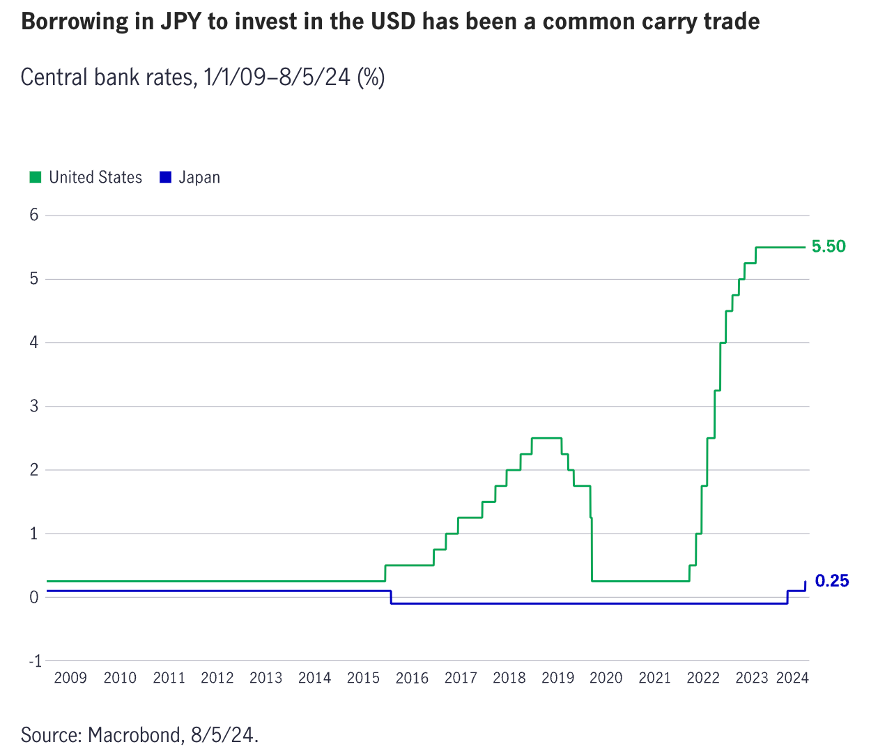
\includegraphics[width=1\linewidth]{Figure1.png}
    \caption{Interest Spread between America and Japan}
    \label{fig:picture1}
    \end{center}
\end{figure}

However, the risk of this kind of carry trade is intrinsic, primarily associated with stock returns and foreign exchange (FX) rates. A decline in American stock return results in lower investment profits. Similarly, a depreciation of the FX rate (i.e., an appreciation of the JPY against the USD) reduces the amount of JPY obtained when converting USD back to repay the loan.  

\subsection{Outline}

In the face of these risks, the proposed product \textbf{Carry Trade Shield} is designed to compensate for the potential losses from the typical carry trade. 

The remainder of this report is organized as follows: Section 2 presents the design of the financial product, including the underlying component and its corresponding payoff function. Section 3 outlines four main processes simulating the interest rates, FX rate and NASDAQ index, followed by parameter calibration. Section 4 provides the results of the product pricing obtained through Monte Carlo simulation, based on the previously defined payoff function and stochastic processes. Finally, Section 5 explores the risk hedging strategy for the product issuer. 

\section{Product Design}

\subsection{Underlying}

The underlying of the product is a functional of the NASDAQ return, which represents the American stock market, and the USD to JPY FX rate. It is assumed that the carry trade investor uses the JPY as the base currency.
At time \(0\), if the FX rate is denoted as \(Y_0\), and the Japanese interest rate is \(r_{B_0}\), then at time \(T\), suppose the return on NASDAQ is \(r_{S_T}\), and the FX rate is \(Y_T\) now. After repaying the borrowed amount, the return on this carry trade is given by the following expression

\[
r_{S_T} \cdot \frac{Y_T}{Y_0} - e^{r_{B_0} T}
\]

\subsection{Payoff Structure}

\[
\Phi(r_{S_{T}}, Y_T) = 
\begin{cases} 
0, & \\
\text{When } r_{S_{T}} \cdot \frac{Y_T}{Y_0} - e^{r_{B_0} T} > 0 \quad (\text{No loss}) 
\\
\\
k \cdot (-0.5) \cdot \left(r_{S_{T}} \cdot \frac{Y_T}{Y_0} - e^{r_{B_0} T}\right), & \\
\text{When } -5\% < r_{S_{T}} \cdot \frac{Y_T}{Y_0} - e^{r_{B_0} T} < 0 \quad \\(\text{Loss but not significant}) \\
\\
-0.5 \cdot \left(r_{S_{T}} \cdot \frac{Y_T}{Y_0} - e^{r_{B_0} T}\right), & \\
\text{When } r_{S_{T}} \cdot \frac{Y_T}{Y_0} - e^{r_{B_0} T} < -5\% \quad \\(\text{Significant loss}) &
\end{cases}
\]

Where \( r_{S_{T}} \cdot \frac{Y_T}{Y_0} - e^{r_{B_0} T} \) is the underlying asset discussed in the previous part, and \(k\) is the proportion of loss that will be compensated.

\[
k = \frac{r_{S_{T}} \cdot \frac{Y_T}{Y_0} - e^{r_{B_0} T}}{-5\%}
\]

\begin{figure}[ht]
    \begin{center}
    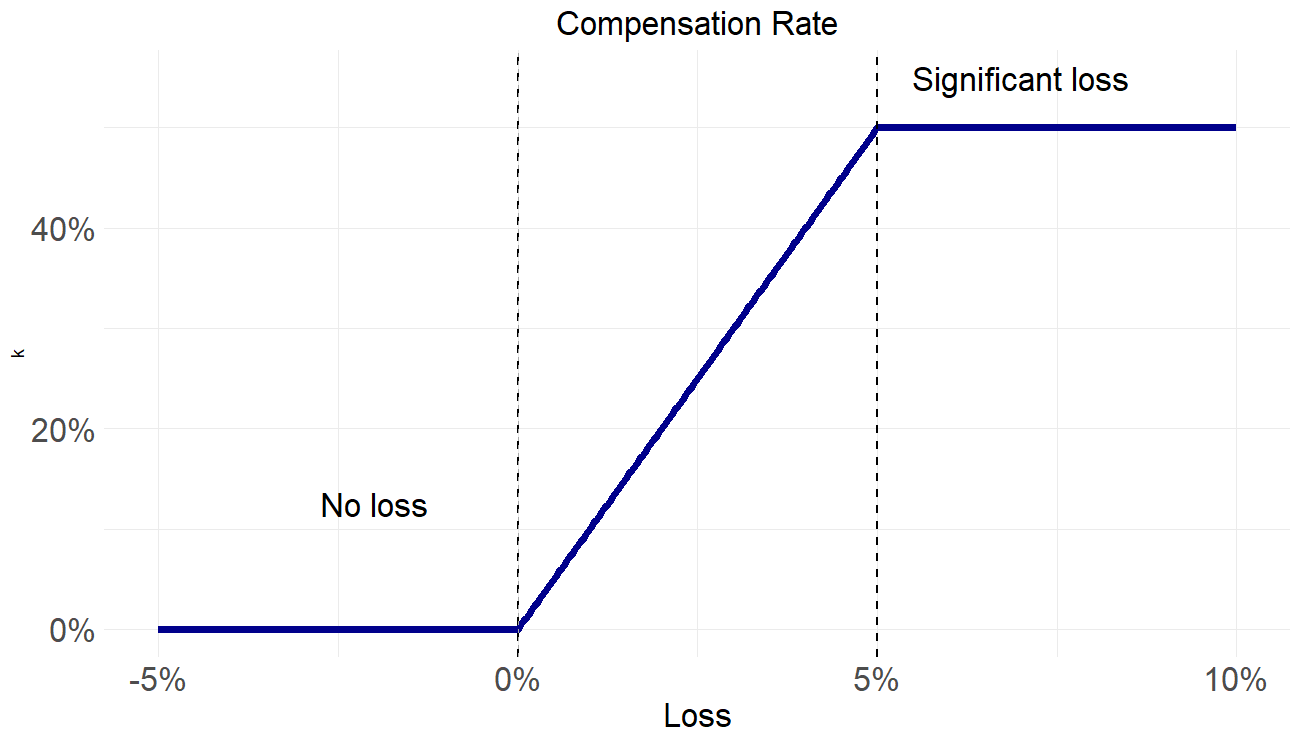
\includegraphics[width=1\linewidth]{Figure2.png}
    \caption{Variation of Compensation Rate \(k\) with Respect to the Underlying}
    \label{fig:picture1}
    \end{center}
\end{figure}

The product is designed for those investors positioned in a carry trade underlying discussed before. By taking our product, investors can significantly decrease their downside risk in case of a negative net return. We try to compensate investors when facing a loss. 

If the net return of the underlying is positive, then there will be no payoff for investors. 

If the net return of the underlying is less than \(-5\%\), which is considered a significant loss, the investor will receive a payment of half the loss. 

If the net return is in a range of \((-5\%, 0)\), then the payoff will be a proportion of the total loss, and the proportion will linearly increase from \(0\) to \(50\%\) when the net return decreases from 0 to \(-5\%\). 

\subsection{Payoff Feature}

Here, \(0\) is designed as a “strike value” to distinguish the range of positive payoff and zero payoff. When the carry trade return is positive, even if it is less than investors’ expectations, investors can take it as an acceptable return. 

When the carry trade return is less than \(-5\%\), the payoff will be \(50\%\) of the loss. This is because there is a significant loss, which is the risk investors want to eliminate.

In this product, \(50\%\) is set as the maximum level of payoff on the underlying because we want to provide more flexibility for investors. Firstly, the product will have a lower price by setting \(50\%\) as the maximum proportion. At the same time investors who wish to take more downside risk and pay less on hedging can take \(50\%\) as hedging and investors who want to take less downside risk, or 0 risks may buy “two products” for “one carry trade” so that it will pay \(100\%\) of the loss when the loss is significant.

When the return of the carry trade is negative but not significant (\(0\) to \(–5\%\)), investors will get a proportion of the loss as the payment. The proportion will increase from 0 to \(50\%\). As discussed before, the idea is that lower loss is more acceptable, and we compensate less and vice versa. At the same time, this payoff diagram can reduce the price significantly so that investors are more likely to buy the product.

\begin{figure}[ht]
    \begin{center}
    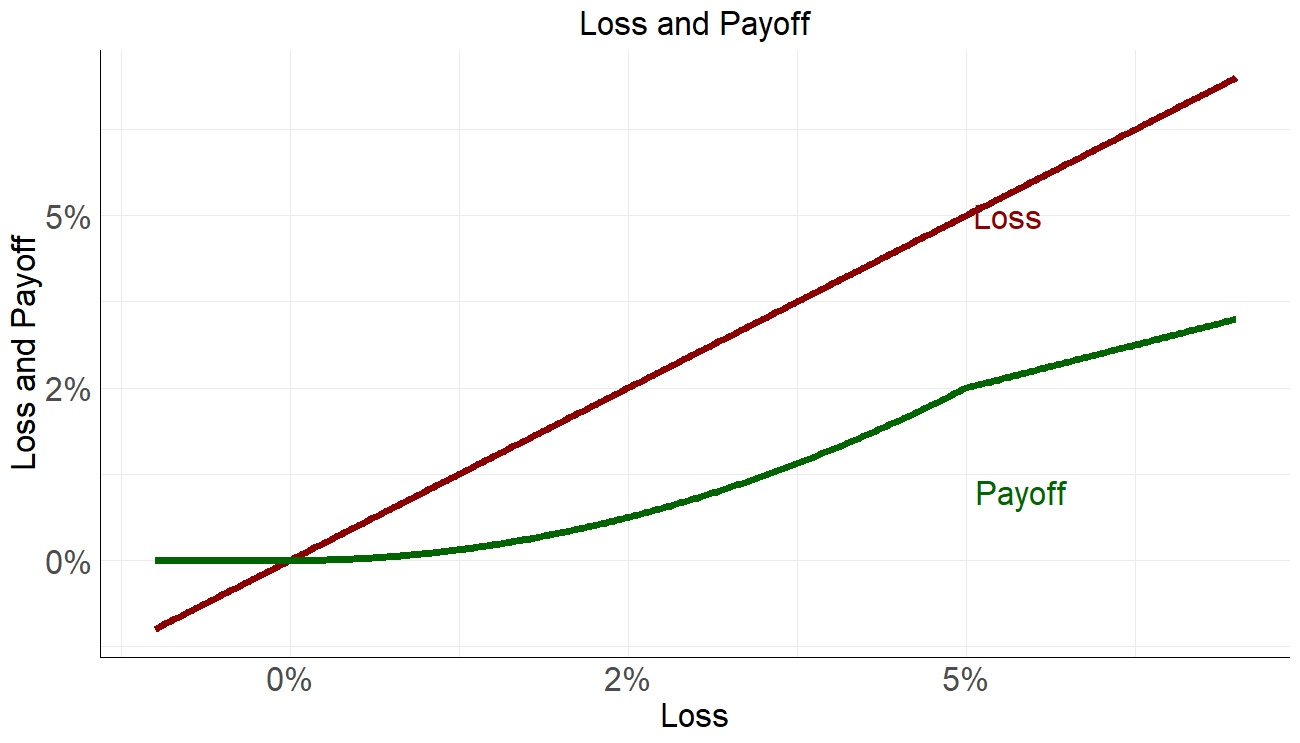
\includegraphics[width=1\linewidth]{Figure3.png}
    \caption{Payoff Structure as a Function of Loss}
    \label{fig:picture1}
    \end{center}
\end{figure}

\section{Modeling and Parameters Estimation}

\subsection{Model Framework}

The foreign exchange rate model is given by the following stochastic differential equation (SDE): 

\[
dY_t = (r_{B_t} - r_{A_t})Y_tdt + \sigma_Y Y_t dW^Y_t
\]

Where: 

\begin{itemize}
    \item $Y_t$ represents the exchange rate between two currencies,
    \item $r_{A_t}$ and $r_{B_t}$ represent the interest rates for countries America and Japan, respectively,
    \item $\sigma_Y$ is the volatility of the exchange rate,
    \item $dW^Y_t$ is a Wiener process driving the randomness of the exchange rate.
\end{itemize}

The drift term $(r_{B_t} - r_{A_t})Y_tdt$ captures the difference in interest rates between the two countries in the risk neutral measure, while the diffusion term $\sigma_Y Y_t dW^Y_t$ captures the random fluctuations in the exchange rate. 

Additionally, the interest rates are modeled using the Vasicek model: 

\[
\text{America: } dr_{A_t} = \kappa_A(\theta_A - r_{A_t})dt + \sigma_A dW^A_t
\]

\[
\text{Japan: } dr_{B_t} = \kappa_B(\theta_B - r_{B_t})dt + \sigma_B dW^B_t
\]

Where:

\begin{itemize}
    \item $r_{A_t}$ and $r_{B_t}$ are short-term interest rates,
    \item $\kappa$ represents the mean-reversion speeds,
    \item $\sigma$ are the volatilities associated with the interest rates.
\end{itemize}

Finally, the stock price process is modeled as:

\[
dS_t = r_{A_t}S_tdt + \sigma_S S_t dW^S_t
\]

\subsection{Estimating the Model Parameters}

To estimate the parameters for the model, historical financial data is required. In this analysis, we used data for the past year from the following sources: 

\begin{enumerate}

    \item US 3-Month Bond Yields,
    \item Japanese 3-Month Bond Yields,
    \item NASDAQ Stock Prices.
    
\end{enumerate}

The following steps are used to estimate the model parameters:

\textbf{Step 1: Calculate DTB3 and Logarithmic Returns}

First, we calculate the 3-month bond yields for the US and the logarithmic returns for the stock prices:
\[
Logarithmic \: Return = \ln\left(\frac{Price_t}{Price_{t-1}}\right)
\]
This transformation helps stabilize variance and makes the data more normally distributed, which is essential for applying statistical models.

\textbf{Step 2: Calculate the Long-Term Mean $\theta$}

Once we have the logarithmic returns for both bond yields and stock prices, we can estimate the long-term mean $\theta$ for the series. This is simply the \textbf{average value} of the series over the observed time period.

\textbf{Step 3: Estimate the Mean Reversion Speed $\kappa$}

The mean-reversion speed $\kappa$ describes how quickly the interest rates return to their long-term means. To estimate $\kappa$, we use a linear regression model. Specifically, we model the change in the interest rate as:
\[
\Delta r_t = \kappa(r_{t-1} - \theta) + noise
\]

\textbf{Step 4: Estimate Volatility $\sigma$}

The volatility $\sigma$ is estimated as the standard deviation of the observed data. It captures the randomness or uncertainty in the process.

\subsection{Data Cleaning and Preprocessing}

To ensure the data is suitable for modeling, we need clean and preprocess the historical datasets. This involves:

\begin{enumerate}

    \item Removing missing or erroneous data points,
    \item Converting the date column into a consistent format,
    \item Sorting the data by date to ensure proper time series analysis.
    
\end{enumerate}

\subsection{Results and Interpretation}

\begin{table}[H]
\centering
\begin{tabular}{|p{1.7cm}|p{1.8cm}|p{1.8cm}|p{2cm}|}
\hline
\textbf{Parameter} & \textbf{America (A)} & \textbf{Japan (B)} & \textbf{Exchange / Stock} \\
\hline
\textbf{$\kappa$} & 0.012994 & -1.235734 & -- \\
\hline
\textbf{$\theta$} & 5.114246 & -0.011982 & -- \\
\hline
\textbf{$\sigma$} & 0.016740 & 0.355882 & \begin{tabular}[c]{@{}c@{}} $\sigma_Y$: 0.007230 \\ $\sigma_S$: 0.010981 \end{tabular} \\
\hline
\end{tabular}
\caption{Estimated Parameters for the Model}
\label{tab:parameters}
\end{table}

It is interesting to note that $\kappa_B$ is negative. However, this might be explained by the Japanese government's decision to \textbf{raise interest rates} on \textbf{2024/03/11} and \textbf{2024/08/01}. The impacts on the rates are as follows:

\begin{itemize}

    \item \textbf{Interest Rate Shocks:} A sudden rise in interest rates can cause unexpected market reactions. Investors, used to low rates, may quickly adjust their portfolios, increasing volatility and pushing rates away from their historical mean. This could result in a negative $\kappa$, as rates diverge instead of reverting to the mean.
    
    \item \textbf{Expectations of Further Rate Hikes:} If the rate increase is seen as the start of a tightening cycle, markets may expect even higher rates. This can reduce bond demand, causing yields to rise further, which might lead to a negative $\kappa$, as rates continue to rise instead of reverting.
    
    \item \textbf{Market Overreaction:} An unexpected rate change can trigger an overreaction, with rapid shifts in rates that do not follow typical mean reversion. This could also lead to a negative $\kappa$, as the rates deviate from the equilibrium due to shock effects rather than gradual reversion.
    
\end{itemize}

Further research on Japanese 3-month Bond Yields during \textbf{March 2023 to March 2024} shows that $\kappa$ is positive (1.380292), suggesting that policy decisions had pushed the data away from its long-term mean.

\section{Pricing Methodology}

\subsection{Simulation Setup and Methodology}

To set a fair price for this product, we use \textbf{Monte Carlo simulation}. The reason for applying Monte Carlo simulation is that the payoff function we derived is piecewise and nonlinear, making it infeasible to obtain analytical solutions. The complexity arises from multiple factors that interact in different ways, such as interest rates, volatility, and asset prices. This combination of nonlinearity and segmentation further underscores the necessity of using a simulation-based approach to accurately estimate the fair price.

In the simulation, term is set $T = 3\,months$ in our simulation. This provides flexibility for investors to readjust their portfolio. $N = 10000000$ iterations are run, generating multiple potential future paths for these variables and their corresponding payoffs. The final price of the product is determined by averaging the payoffs across all simulated scenarios.


\subsection{Simulation Results}

\begin{figure}[ht]
    \begin{center}
    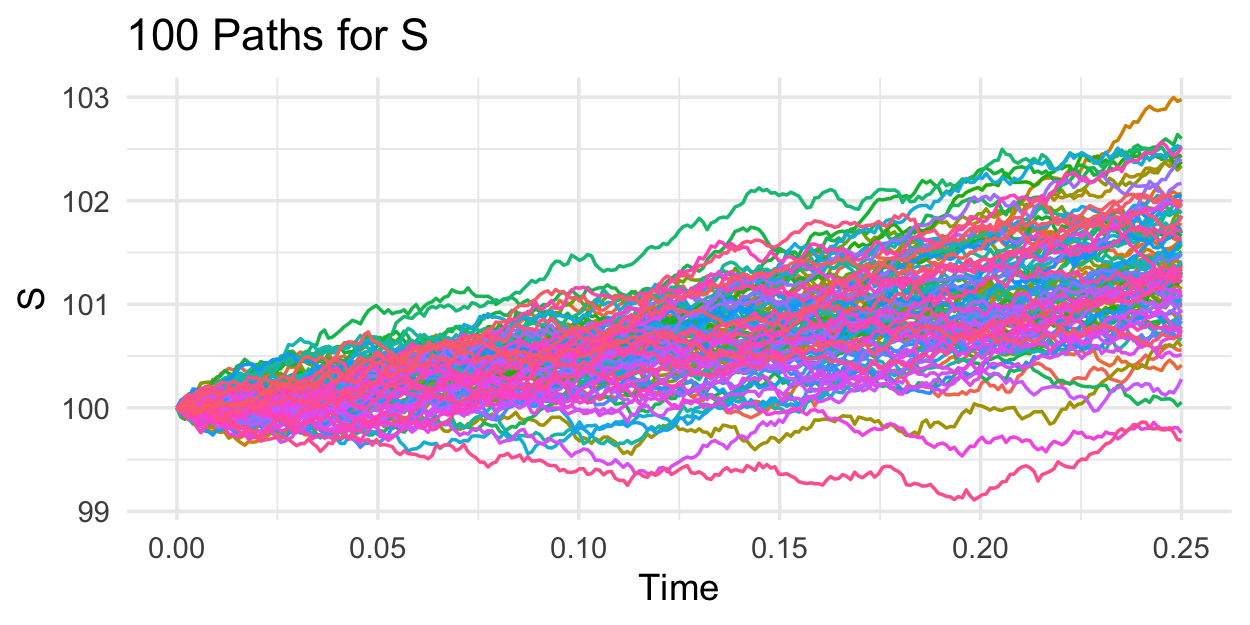
\includegraphics[width=1\linewidth]{Figure4.png}
    \caption{Possible Paths for NASDAQ}
    \label{fig:picture1}
    \end{center}
\end{figure}

\begin{figure}[ht]
    \begin{center}
    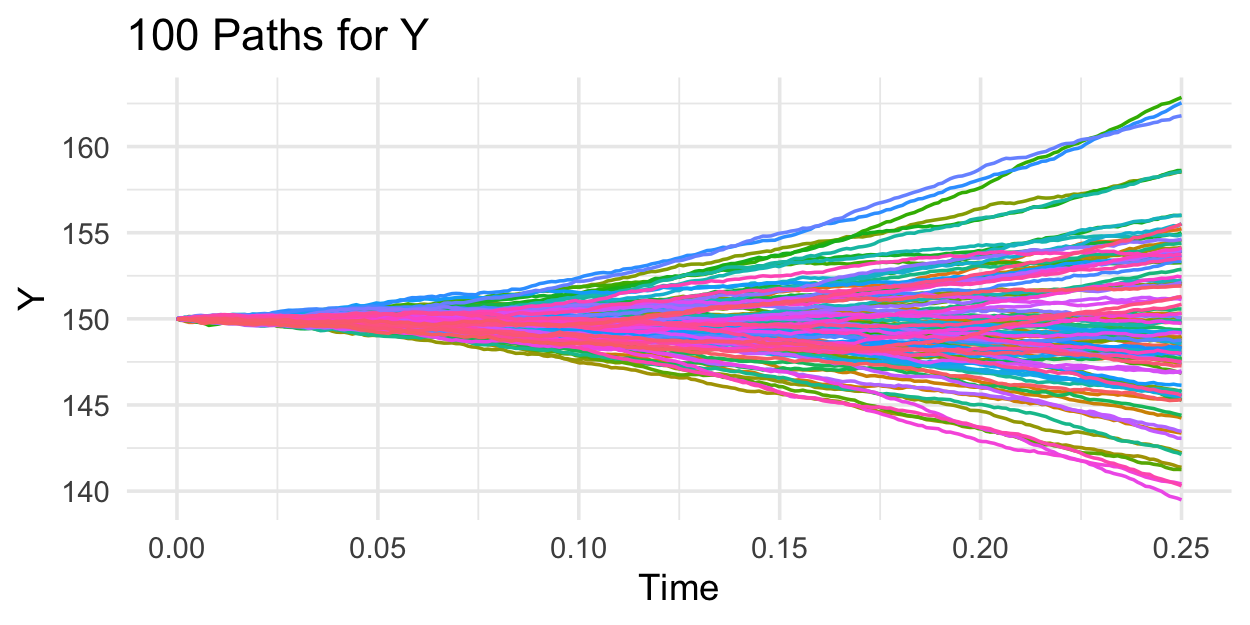
\includegraphics[width=1\linewidth]{Figure5.png}
    \caption{Possible Paths for Exchange Rate}
    \label{fig:picture1}
    \end{center}
\end{figure}

The 2 graph above shows 100 paths for NASDAQ and FX rates over the product horizon, respectively. This illustrates 100 possible scenarios for the underlying.

\begin{figure}[ht]
    \begin{center}
    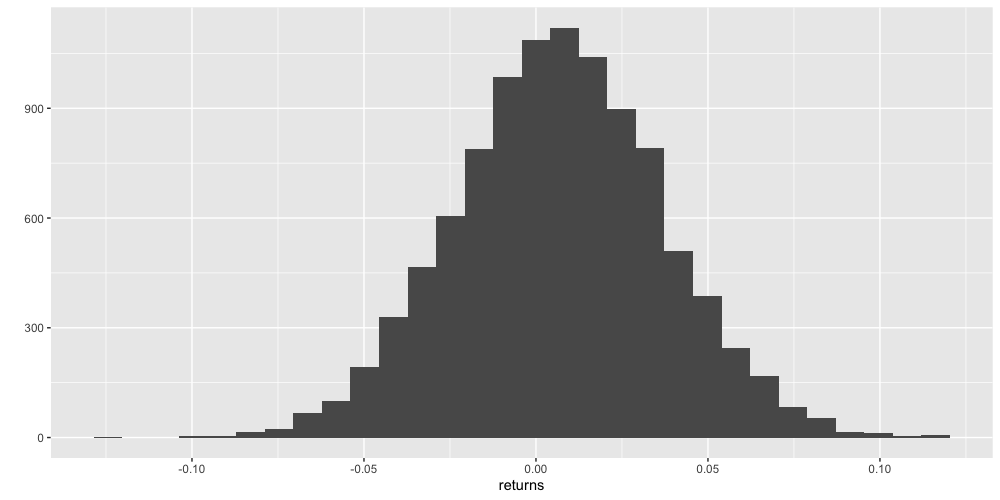
\includegraphics[width=1\linewidth]{Figure6.png}
    \caption{Histogram of the Returns of Carry Trade Investors}
    \label{fig:picture1}
    \end{center}
\end{figure}

The graph presented here is a histogram of the returns of carry trade investors. The distribution is almost symmetric and in a bell shape. It has a mean slightly above zero. This indicates that the more than half of the scenarios simulated, American stocks returns outperform Japanese borrowing rate. 

\begin{figure}[ht]
    \begin{center}
    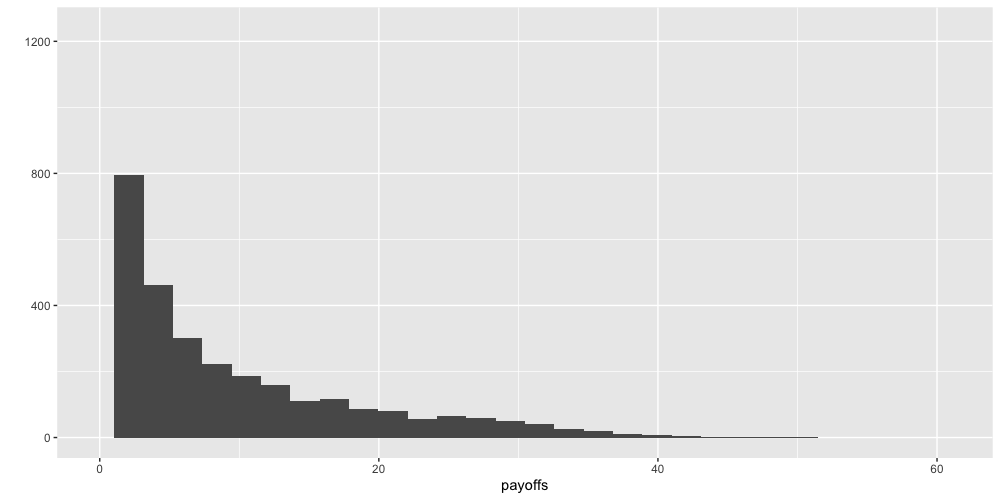
\includegraphics[width=1\linewidth]{Figure7.png}
    \caption{Payoff Distribution}
    \label{fig:picture1}
    \end{center}
\end{figure}

The payoff distribution diagram for the product shows a descending trend in frequency for larger payoffs. This indicates that the probability of increasingly negative payoff is rare, and so does the compensation from this product. This product will never generate loss, as it is designed to compensate investors if they incur loss in their carry trade.

\subsection{Pricing from Simulation Results}

After the simulation, the product is estimated to be \textbf{3.7054}, based on a principal investment of \textbf{1,000}. This suggests that investors need to pay about \textbf{0.37\%} of their principal to hedge half their significant negative returns, or \textbf{0.74\%} of the principle investment to cover all of their significant loss. It might serve as an insurance in their carry trade, if they encounter significant loss.

\section{Risk Hedging For Product Issuer}

Banks need to adopt effective hedging strategies in risk management in order to realize the robustness of product returns. In the absence of an analytical solution, this section uses the Delta approach of sensitivity analysis to quantitatively assess and hedge risk. Specifically, by measuring the impact of key variables such as \textbf{Equity Price Delta} and \textbf{Foreign Exchange Rate Delta} on product performance, it is possible to accurately assess potential risks and formulate mitigation strategies accordingly. These quantitative indicators are of great significance in product risk management, providing theoretical basis and practical support for achieving the goal of robust returns.

\subsection{Equity Price Delta}

Equity Price Delta measures the impact of equity price volatility on portfolio value. By using the centered difference method, the equity price is adjusted by a small increment ($\pm 0.5h$), and the resulting product payoff changes are averaged to derive the equity price delta.

\begin{align*}
\Delta_{\text{Equity}} &\approx \frac{\Pi(t, (1 + 0.5h)S, Y; X) - \Pi(t, (1 - 0.5h)S, Y; X)}{hS} \\
&\approx -1.9160
\end{align*}

In this analysis, the delta is calculated as $-1.9160$ at $S = 100$, indicating that the payoff of the product is negatively correlated with equity price increases. Specifically, a negative delta implies that the seller of the product incurs losses as equity prices drop, revealing exposure to market dynamics.

This result has important practical implications. A negative equity delta highlights the need to hedge against dropping equity prices to maintain product stability. This can be achieved through the following strategies:

\begin{itemize}

    \item \textbf{Short Selling the Equity (ETF)}: Enter into short positions in the equity or its ETF. Gains from these positions offset losses in the portfolio if equity prices drop.

    \item \textbf{Purchasing Put Options on Equity}: Acquire put options, which grant the right to sell underlying ETF or indices at a predetermined price. These options generate intrinsic value as equity prices decrease, offsetting potential losses in the product.
    
\end{itemize}

\subsection{Foreign Exchange Rate Delta}

Foreign Exchange Rate Delta measures the sensitivity of the product payoff to changes in foreign exchange (FX) rates. Similar to the equity price delta calculation, the central difference method is applied to assess this impact. The FX rate is adjusted by a small increment ($\pm 0.5h$), and the resulting product changes are averaged to derive the FX delta.

\begin{align*}
\Delta_{\text{FX}} &\approx \frac{\Pi(t, S, (1 + 0.5h)Y; X) - \Pi(t, S, (1 - 0.5h)Y; X)}{hS} \\
&\approx -1.2516
\end{align*}

In this analysis, the calculated delta is $-1.2516$ at $Y = 150$, indicating a negative correlation between the product payoff and FX rate increases. Specifically, a negative FX delta suggests that the bank loses when foreign exchange rates drop. This highlights a significant exposure to JPY depreciation relative to the USD.

A negative FX delta can be hedged using the following methods:

\begin{itemize}

    \item \textbf{Buying the JPY}: Purchase the JPY directly in the FX market. This creates gains when the JPY appreciates (or the USD depreciates), offsetting losses in the product's payoff.

    \item \textbf{Using Currency Options}: Purchase put options on the USD. These options provide the right to sell the USD at a predetermined rate, mitigating the impact of adverse currency movements. Alternatively, call options on the JPY can achieve a similar hedging effect.

\end{itemize}

\subsection{Practical Application of Dynamic Risk Management}

The dynamic risk management insights derived from the sensitivity analysis are practical and actionable. These insights provide a structured approach to implementing a dynamic hedging strategy. Deltas serve as a guide for adjusting exposures, enabling banks to precisely optimize hedging allocations.

This approach contributes to the stabilization of the portfolio. By dynamically adjusting the hedging positions in accordance with the computed Deltas, the portfolio's sensitivity to market volatility is significantly reduced, thereby promoting consistent and stable returns.

\section{Conclusion}

\subsection{Summary of Findings}

This study introduces the \textbf{Carry Trade Shield}, a structured financial product designed to mitigate risks in carry trade strategies. By combining stochastic modeling and Monte Carlo simulations, the product provides a cost-effective way to manage currency and equity volatility risks. The results demonstrate its effectiveness in reducing downside exposure for investors while ensuring affordability.

\subsection{Data and Code Accessibility}

The data for this project, as well as the code for data cleaning, parameter estimation, model simulation, and delta calculating is open-source and available on GitHub. Interested readers and practitioners can access the repository via the following link: \href{https://github.com/lststar/Carry-Trade-Shield}{https://github.com/lststar/Carry-Trade-Shield}.

\begin{thebibliography}{4}

\bibitem{Investing}
Investing.com. History stock price and interest rate. Retrieved from \href{https://www.investing.com/}{https://www.investing.com}

\bibitem{Ahlip2013}
Ahlip, R., Rutkowski, M. (2013). Pricing of foreign exchange options under the Heston stochastic volatility model and CIR interest rates. Quantitative Finance, 13(6), 955–966.
\href{https://doi.org/10.1080/14697688.2013.769688}{https://doi.org/10.1080/14697688.2013.769688}

\bibitem{Bergomi2016}
Bergomi, L. (2016). Stochastic volatility modeling. Boca Raton, FL: CRC Press.

\bibitem{Gulisashvili2012}
Gulisashvili, A. (2012). Stock price models with stochastic volatility. In Analytically tractable stochastic stock price models (pp. 25–80).
\href{https://doi.org/10.1007/978-3-642-31214-4_2}{https://doi.org/10.1007/978-3-642-31214-4\_2}


\end{thebibliography}

\end{document}